\documentclass[12pt]{article}


\usepackage{EngReport}
\usepackage{amssymb}


\graphicspath{{Images/}}
\bibliography{Sources}
%%\onehalfspacing
\singlespacing
\graphicspath{{images/}}
\geometry{letterpaper, portrait, includeheadfoot=true, hmargin=1in, vmargin=1in}

%\fontsize{font size}{vertsize (usually 1.2x)}\selectfont

\begin{document}
\renewcommand{\familydefault}{\rmdefault}

\begin{titlepage}
    \centering
    {
\includegraphics[width=0.2\textwidth]{Images/fiuner.png}\par}
    \vspace{1cm}
    {\bfseries\LARGE Universidad Nacional de Entre Ríos \par}
    \vspace{1cm}
    {\scshape\Large Facultad de Ingeniería \par}
    \vspace{3cm}
    {\scshape\Huge Trabajo Integrador Final\par}
    \vspace{0.5cm}
    {\itshape\Large TIC Y Geomática \par}
    \vfill
    {\Large Autor: \par}
    {\Large Justo Garcia \par}
    \vfill
    {\Large Junio 2024 \par}
\end{titlepage}

\graphicspath{{Images/}}
\pagestyle{fancy}
\fancyhf{}
\setlength{\headheight}{30pt}
\renewcommand{\headrulewidth}{0.4pt}
\renewcommand{\footrulewidth}{0.4pt}
\lhead{TIF \\ TIC y Geomática }
\rhead{2024 \\ Garcia Justo}
\rfoot{\textbf{\thepage}}
\lfoot{
\includegraphics[scale=0.07]{Images/fotouner.png}}
\renewcommand*\contentsname{Tabla de contenidos}
\tableofcontents
\pagebreak

% % % % % % % % % % % % % % % % % % %
% % % % %  SAMPLE IMAGE   % % % % % %https://www.overleaf.com/project/64eb940f11b4d5805e560df5
% % % % % % % % % % % % % % % % % % %


% \begin{figure}[h]
%     \centering
%     \includegraphics[width=.95\linewidth]{example-image-a}
%     \caption{** Concept Image Caption **}
%     \label{fig:my_label}
% \end{figure}

% % % % % % % % % % % % % % % % % % % %
% % % % %  REPORT CONTENT   % % % % % %
% % % % % % % % % % % % % % % % % % % %

\fontsize{12}{20}\selectfont{

\singlespacing
\section{Introducción}

El presente informe detalla un proyecto realizado en el marco del cursado de la materia TIC y Geomática de la Facultad de Ingeniería de la Universidad Nacional de Entre Ríos, enfocado en el análisis de la distribución espacial de vectores del dengue utilizando tecnologías geoespaciales y análisis de imágenes satelitales. Todas las técnicas utilizadas en este proyecto tienen como objetivo extraer la información necesaria para aplicar un método numérico concreto de la bibliografía. Aunque se plantea la resolución matemática del modelo como una proyección futura, las técnicas y procedimientos de extracción, obtención y procesamiento de los datos necesarios para ello se implementan y explican detalladamente en este informe.

El dengue, una enfermedad transmitida por mosquitos del género Aedes, representa un desafío significativo para la salud pública. El estudio de la distribución de estos vectores es esencial para la implementación de estrategias. La combinación de datos satelitales y herramientas geoespaciales permite explorar como diferentes factores afectan la proliferación de los mosquitos.

El objetivo principal de este proyecto es aplicar los conocimientos adquiridos en la materia en una problemática real. A partir de la búsqueda bibliográfica se plantea la replicación en un área de interés diferente (Oro Verde, Entre Ríos, Argentina) de un trabajo que caracteriza y modela la distribución espacial de los vectores del dengue.

Este informe detalla el proceso desde la obtención de imágenes satelitales hasta el procesamiento geoespacial de los datos, incluyendo la delimitación del área de estudio, la extracción y análisis de índices espectrales como el NDVI y NDWI, así como la clasificación de superficies utilizando técnicas avanzadas en el análisis de datos geoespaciales. La implementación práctica del modelo matemático se deja como una proyección futura, mientras que el foco actual está en la preparación de los datos necesarios para este propósito.


\section{Desarrollo}

\subsection{Área de estudio}

Se contaba con datos de ovitrampas de un proyecto proveniente de la Facultad en Oro Verde, para definir el área de interés se llevó a cabo un procesamiento en Python con Folium y Pandas, esto permitió obtener gráficas sobre los puntos geográficos en los que teníamos información de densidad de mosquitos.
	
\begin{figure}[H]
	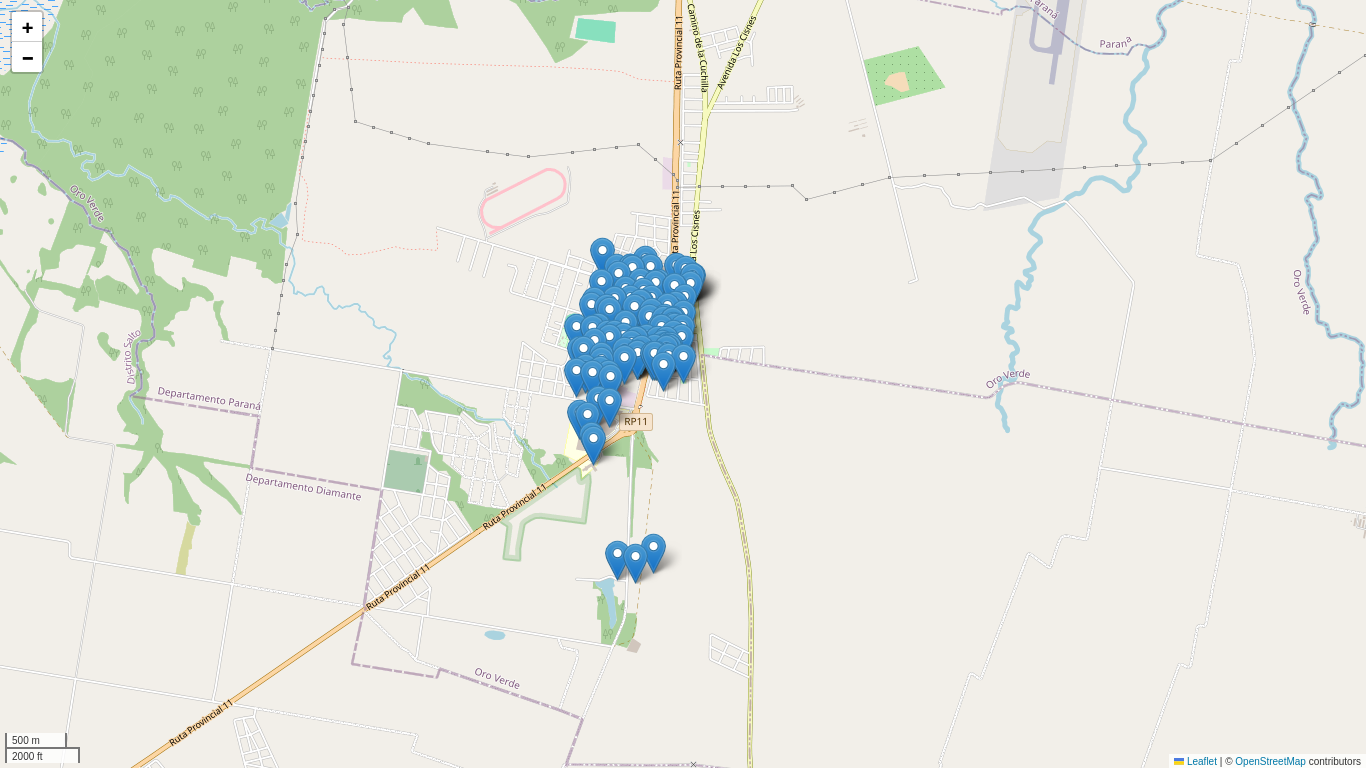
\includegraphics[width=0.7\textwidth]{ovitrampas.png}
	\centering
	\caption{Posiciones de ovitrampas en Oro Verde.}
	\label{fig:ovitrampas}
	
\end{figure}



%% Podría ser buena idea agregar una foto del área de interés desde distintas perspectivas, una en la proyección mundial, otra en el mapa y después directamente la imágen.


\subsection{Obtención de imágenes}

\subsubsection{Dispositivo de sensado}

\subsubsection{Análisis visual}

\subsection{Descripción del modelo}

$$\frac{\partial \rho(P,t)}{\partial t}=\bigtriangledown .(D_R \bigtriangledown \rho)-\bigtriangledown.(\rho D_W V)- \bigtriangledown . (\rho K_H \bigtriangledown H) + \alpha - \beta$$

Donde:

\begin{center}
	\begin{tabular}{|c | c | c|} 
		\hline
		\textbf{Símbolo} & \textbf{Variable} & \textbf{Valor}\\
		\hline
		$$P$$ & Densidad de mosquitos & No homogéneo \\
		\hline
		$\alpha$  & Tasa de nacimientos & $6 (m^2/dia)$ \\
		\hline
		$\beta$  & Tasa de muertes             & 0.2 \\
		\hline
		$V$   & Velocidad Viento Superficie & No homogéneo \\
		\hline
		$K_H$   & Tensor de atracción         & 100 \\
		\hline
		$H$    & Campo de atracción          & No homogéneo \\
		\hline
		$D_R$   & Tensor de difusión          & No homogéneo / ver Tabla 2 \\
		\hline
		$D_W$   & Tensor de rugosidad         & No homogéneo / ver Tabla 2\\
		\hline
	\end{tabular}
\end{center}



\section{Conclusiones}


}

\pagebreak

\printbibliography[title={Referencias}]

\end{document}
